\documentclass[12pt]{article}  % 官方要求字号不小于 12 号,此处选择 12 号字体

% 本模板不需要填写年份,以当前电脑时间自动生成
% 请在以下的方括号中填写队伍控制号
\usepackage[2020987]{easymcm}  % 载入 EasyMCM 模板文件
\problem{C}  % 请在此处填写题号
\usepackage{mathptmx}  % 这是 Times 字体,中规中矩 
\usepackage{graphicx}
\usepackage{float}
\usepackage{subfigure}
%\usepackage{mathpazo}  % 这是 COMAP 官方杂志采用的更好看的 Palatino 字体,可替代以上的 mathptmx 宏包
\usepackage{fontspec}
\setmainfont[
BoldFont=Adobe Garamond LT Bold.ttf,
ItalicFont=Adobe Garamond LT Italic.ttf,
BoldItalicFont=Adobe Garamond LT Bold Italic.ttf
]{Adobe Garamond LT Regular.ttf}

\title{\textbf{Learning Sale Strategy from Amazon Historical Data}}  % 标题

% 如需要修改题头(默认为 MCM/ICM),请使用以下命令(此处修改为 MCM)
%\renewcommand{\contest}{MCM}

% 文档开始
\begin{document}
% 此处填写摘要内容
\begin{abstract}
With the rapid development of Internet technology, the business industry is also gradually shifting to the O2O (online to offline) model . How to keep products attractive to consumers has become an inevitable problem for many companies. In this article, we have established a product appraisal model for Sunshine and given our recommended online sales strategy.

In order to provide the best strategy for online sales, we analyze the data provided by Sunshine Company and provide the following suggestions:

First, we used the \textbf{FAHP} model to evaluate the weight of each index in the review. We found that compared to ``Review Date'' and "Total votes", ``Helpful votes'', ``Star ratings'', and ``Verified purchase'' are more informative. However, the FAHP model is kind of subjective, and information quantity is probably affected by review contents. In order to better confirm the value of reviews, we rank them using a method based on the weighted gray correlation degree.

Second, with time-based \textbf{SARIMA} model to forecast the sales time series, we find that the products which have great star ratings and large sales amount in history have more potential to continue performing better in the future. However, only using the sales amount is not scientific or accurate enough. We also find several products performed well in the previous period of time but are not likely to have considerable sales in the future. Sales data in the most recent years seems more significant.


Third, we generate dependencies representation to extract sentimental adjectives and adverbs from comments for sentiment analysis. With our statistics result, we find that negative words and adversative conjunctions are more probable to be found in negative comments and positive words are more probable to be found in positive ones. Some neutral words which have no exact meanings appear in high frequency in all comments. However, some positive words also have high frequency in negative reviews. So using negative and adversative conjunctions to predict a bad performance seems more reasonable. Furthermore, we use \textbf{ABSA} model to give more accurate suggestions about which aspects need more attention of each products.


Fourth, by combining star ratings, helpful votes, total votes and reviews, we generate a precise score called \textbf{``Predict Score" }to evaluate a product accurately. Since in real situations, we can not obtain helpful votes and total votes in time. If  we would like to make a real-time evaluation, we can only use limited star ratings and reviews. In our model, the ``Predict Score", fit by history vote data, is compounded by star ratings and review scores with dynamic coefficients and  without any delay.


Finally, we perform sensitivity analysis on the established evaluation system and change the index weights to check our model's robustness.


In summary, we have established a product scoring system that can provide companies with a market estimate of products in advance.

    % 美赛论文中无需注明关键字。若您一定要使用,
    % 请将以下两行的注释号 '%' 去除,以使其生效
    %\vspace{5pt}
    %\textbf{Keywords}: MATLAB, mathematics, LaTeX.

\end{abstract}

\maketitle  % 生成 Summary Sheet
\tableofcontents  % 生成目录


% 正文开始
\section{Introduction}
\subsection{Problem Background}
Before, you may be new to "data mining" and may be surprised at the "bag of words model". However, with the advent of the era of big data, it seems that nowadays it's of great importance for companies to get hang of the prospect of products before launching, aiming to archive most profit. Sunshine intends to improve online sales strategies for new products and increase customer satisfaction. Here we studied meaningful quantitative and qualitative relationships within and between star ratings, reviews, and helpfulness ratings to help Sunshine succeed in three new products.

Two major problems are discussed in this paper, which are:
\begin{itemize}
    \item How to combine ratings and reviews to analyze changes in product reputation and predict future sales, so as to choose the best online sales strategy.
    \item How to combine ratings and reviews to find a comprehensive model that best reflects product conditions and consumers' needs, so as to evaluate potential success or failure and identify potentially important design features.
\end{itemize}

%\subsection{Literature Review}
%A literatrue\cite{1} has used conjunction for sentiment analysis for product reputation evaluation. The %author studied the impact of conjunction and introduced conjunction classification based on sentiment %analysis. The proposed sentiment analysis method incorporates all sentiment bearing parts of speech to %find the polarity.


\subsection{Our work}
Our work can be divided into five parts.
\begin{enumerate}
    \item Data preprocess. We extract users' data of the three  products from a glossary of data label definitions, and performed data filtering based on the characteristics of the data to provide easy-to-handle data for subsequent data analysis.
    \item Index priority. We use the fuzzy analytic hierarchy process to give initial weight to relative parameters, establish a basic model based on users' star ratings, reviews, and helpfulness votes, aiming to aid Sunshine Company be aware of the prior data indexes.
    \item Sentiment analysis. We conduct sentiment analysis to discuss reviews' polarity and found the relations between words and comments. Moreover, we applied ABSA for more accurate suggestions.
    \item Predict score.  We construct a model which is used for the generator of "Predict Score" ,a evaluation index of products' performance .
    \item Sensitivity analysis. We perform sensitivity analysis on the established scoring system and change the index weights to have a robustness check.
    
    
\end{enumerate}


In summary, we have established a model to help Sunshine Company get more acquainted with the products' sales market on the basis of former products' data. At the same time, we also investigated the design characteristics of previous well-sold products and the fluctuation laws of sales, and provided Sunshine Company with some suggestions on sales strategies and products' feature design.

\section{Assumptions and Notations}
\subsection{Assumptions}     
\begin{enumerate}[\bfseries 1.]
    \item The given data is sufficient to get the trend of the data over time, so it can be predicted by a time series model.
    \item The initial weight of each parameter has negligible effect on the model. Therefore, it is possible to assign weights using the method of analytic hierarchy process.
    \item The unconfirmed purchase data is not used in our further model because it only accounts for a small part of the data and contains too many innumerable influence factors.
\end{enumerate}

\subsection{Notations}
The primary notations used in this paper are listed in Table \ref{tb:notation}.
\begin{table}[!htbp]
\begin{center}
\caption{Notations}
\begin{tabular}{cl}
	\toprule
	\multicolumn{1}{m{3cm}}{\centering Variable}
	&\multicolumn{1}{m{8cm}}{\centering Definition}\\
	\midrule
	$h_v$& Number of helpful votes for single product\\
	$t_v$& Number of total votes for single product\\
    $w_1$& Weight of star rating\\
	$w_2$& Weight of review score\\
	$m$  & Number of the observation per year\\
    $p$  & Order of the autoregressive part\\
    $d$  & Degree of first differencing involve\\
    $q$  & Order of the moving average part\\
    $P$  & Seasonal order of the autoregressive part\\
    $D$  & Seasonal degree of first differencing involved\\
    $Q$  & Seasonal order of the moving average part\\
	\bottomrule
\end{tabular}\label{tb:notation}
\end{center}
\end{table}

\section{Model design}


\subsection{Data Prepossessing}
Why data processing? First, the amount of original data is large and it is very inconvenient to process. Second, the original data contains a lot of redundant and invalid data, which will cause a lot of interference to our model building. So data preprocessing is essential.

\subsubsection{Data Cleaning and Visualization}
Data Cleaning is the first step in data preprocessing. In order to improve the accuracy of the data and lie the foundation for subsequent data processing, we filter out redundant data in the original data, such as unconfirmed purchases or those time of purchase earlier than 2008, etc., In our model, we only discuss customers data between 2008 and 2015.

From the following two figures(Figure \ref{fig:count rating} and Figure \ref{fig:count rating eight years}), we can see that the data after data filtering has not changed much in star ratings, so it illustrates the feasibility of data filtering. From the bar chart it is evident that most of the customers give 4 or 5 star ratings to these products. At the same time, we can see that the total sales amount goes higher and higher as time goes by, this may caused by either the development of the economy or the result of advertising. We will do further analysis later.

\begin{figure}[!htbp]
\centering
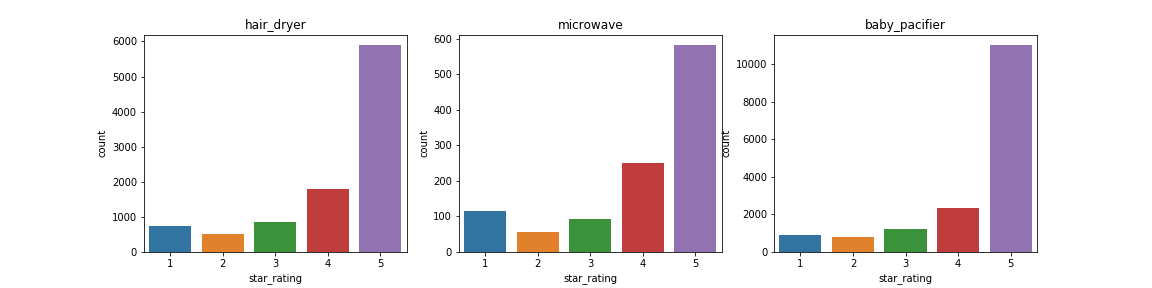
\includegraphics[width=.8\textwidth]{count_rating.png}
\caption{Number of total Star Ratings}\label{fig:count rating}
\end{figure}

\begin{figure}[!htbp]
\centering
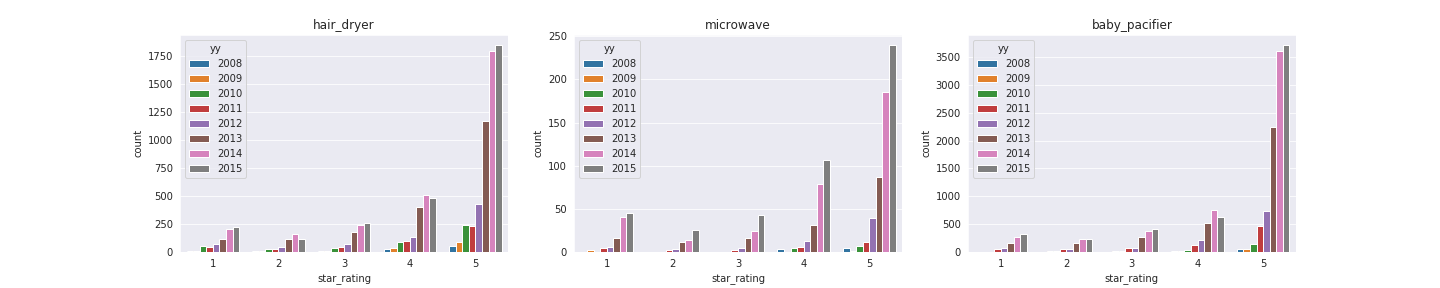
\includegraphics[width=.8\textwidth]{count_rating_8year.png}
\caption{Number of Star Ratings by Year}\label{fig:count rating eight years}
\end{figure}

Figure \ref{fig:Rating mean} is the variation of mean star ratings of total products by category. From the figure, we can find that the ratings of hair dryer and baby pacifier are relatively stable but the score of microwave seems have a large fluctuation especially in 2009. After referring to the raw data, we find that this is because the sales amount is small compared with baby pacifier and hair dryer. Moreover, all of the three product have a good star rating in the nearest 5 years.
\begin{figure}[!htbp]
\centering
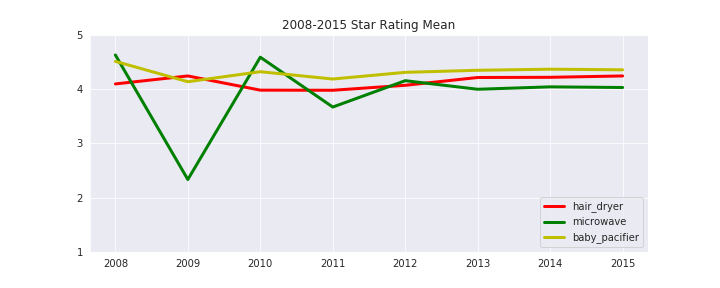
\includegraphics[width=.8\textwidth]{Rating Mean.png}
\caption{Mean of Star Ratings by Year}\label{fig:Rating mean}
\end{figure}

\subsubsection{Filtering Information from Reviews}
Sentiment analysis is an automatic method to find the opinion of a person about a product. Recently, it is a hot research field of natural language processing, computational linguistics and text mining. \cite{1}

First, we will count the total reviews by year, it is understandable the reviews also go up by year becasue of the rise of sales amount. The results of products' comments are shown in Figure \ref{fig:comment}.\\

\begin{figure}[H]
\centering
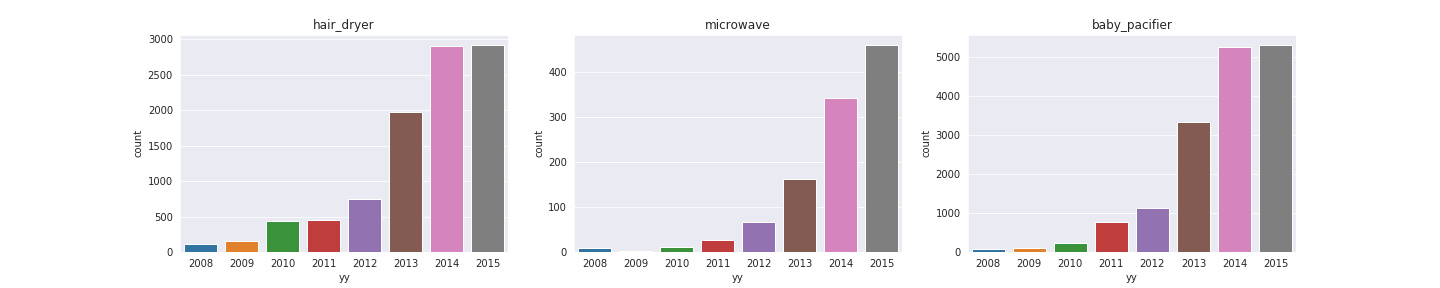
\includegraphics[width=.8\textwidth]{count_comment_8year.png}
\caption{Number of Review by Year}\label{fig:comment}
\end{figure}

Next, we clean the review by merging the headline and review body, remove the punctuation and remove the "Stopwords". Then, we make a rough words statistics by generating a "Word cloud" to show some high-frequency positive and negative words in order to get familiar with those reviews.  

\begin{figure}[!htbp]
\centering
\subfigure[Positive]{
\begin{minipage}[t]{0.5\linewidth}
\centering
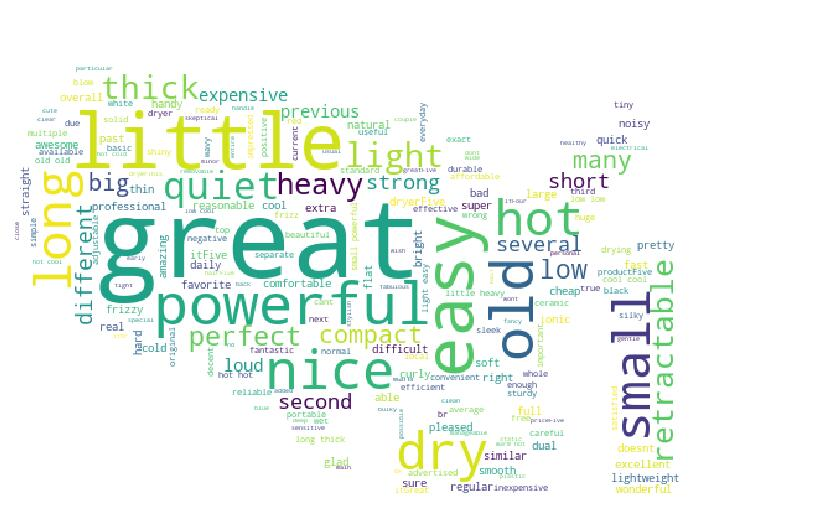
\includegraphics[width=4in]{positive word cloud.jpg}
%\caption{Positive}
\end{minipage}%
}%
\subfigure[Negative]{
\begin{minipage}[t]{0.5\linewidth}
\centering
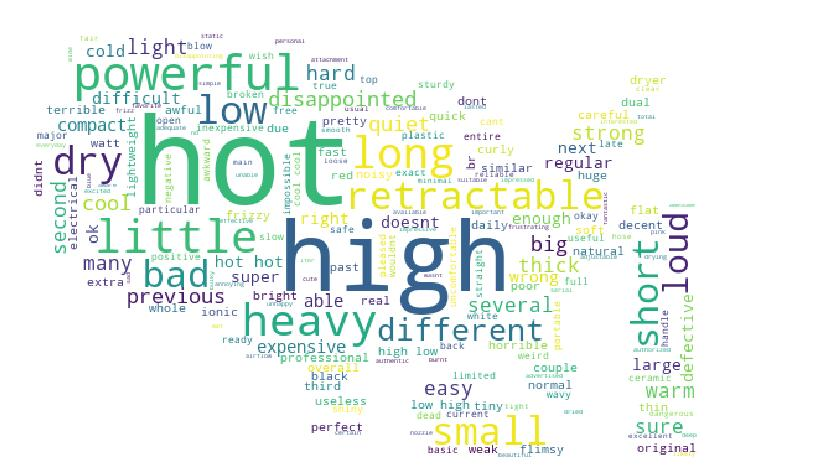
\includegraphics[width=4in]{negative word cloud.jpg}
%\caption{Negative}
\end{minipage}%
}%
\centering
\caption{Word Cloud}
\end{figure}




\subsection{Basic Model}


\subsubsection{Data Analytic with FAHP}

To pick the best profile, we adopted Fuzzy Analytic Hierarchy Process (FAHP) as the assessment model. FAHP is a multi-objective decision analysis tool, which is used to analyze multi-attribute decision-making problems, based on Analytic Hierarchy Process (AHP). It represents an accurate approach for quantifying the weights of decision criteria\cite{2}. 
% 这里需要换参考文献为张吉军那篇

The model is composed of three parts: index, criteria and goal. The goal consists of the best weight distribution scheme, and the criteria is used for deciding priority two by two.


Based on experience,  we chose four representative indexes as elements in criteria: 
\begin{enumerate}[\bfseries 1.]
    \item Star rating. It visually illustrates the quality of the product. Customers are able to get the information at the first glance. 
    \item Helpful votes. Obviously, a review are  more convincing with more helpful votes.
    \item Total votes. A review may be more informative if it gets many votes.
    \item Verified purchase. If a customer buy the product at a discount, he or she may psychological expectations and gives higher rating because of the low price. 
    \item Review date. Reviews from recent transactions may better reflect the quality of the products, as these products were produced during the same period.
\end{enumerate}


The FAHP hierarchy is shown in the following figure.

\begin{figure}[!htbp]
\centering
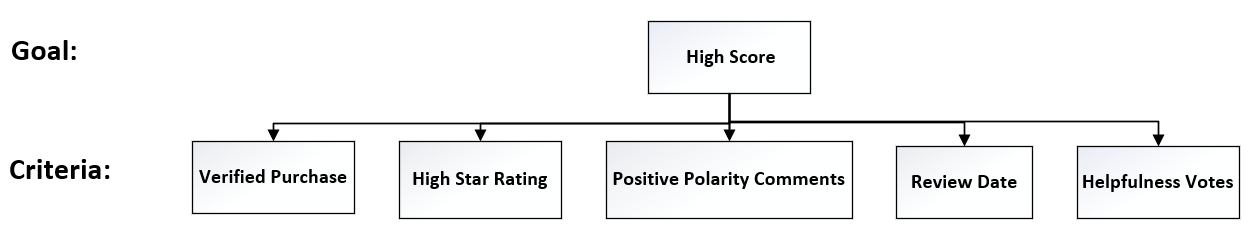
\includegraphics[width=.6\textwidth]{e.PNG}
\caption{FAHP}\label{fig:FAHP}
\end{figure}

By the following function, we obtained the comparison matrix A.

\begin{equation}\label{eq:1}
a_{ij} = \begin{cases}
        1,   &\text{if }\ a_i \text{ is more important than}\ a_j  \\
        0.5, &\text{if } a_i \text{ and }\ a_j \text{ have the same importance}\  \\
        0,  &\text{if }\ a_j \text{ is more important than }\ a_i
        \end{cases}
\end{equation}


\begin{figure}[!htbp]
\centering
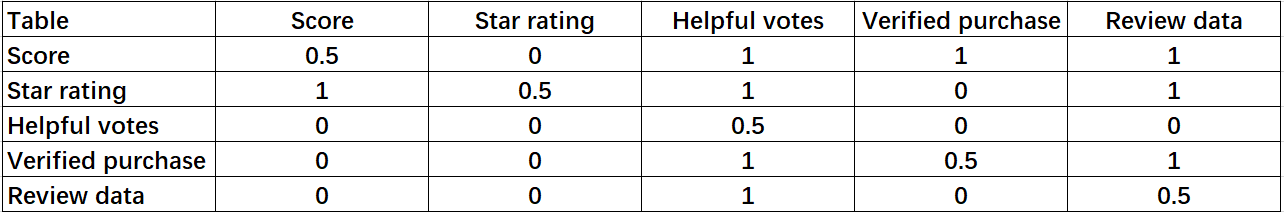
\includegraphics[width=.6\textwidth]{z.png}
\caption{Comparison Martix}\label{fig:Comparison Matrix}
\end{figure}

By these following functions, we transformed the comparison matrix into the fuzzy consistency matrix B below.

\begin{equation}\label{eq:1}
a_i = \sum\limits_{j=1}^{n} a_{ij}  \quad i=1,2,3,...n
\end{equation}

\begin{equation}\label{eq:2}
a_j = \sum\limits_{i=1}^{n} a_{ij}  \quad j=1,2,3,...n
\end{equation}

\begin{equation}\label{eq:3}
b_{ij} = \frac{a_i-a_j} {2n} + 0.5  \quad i,j=1,2,3,...n
\end{equation}


\begin{figure}[!htbp]
\centering
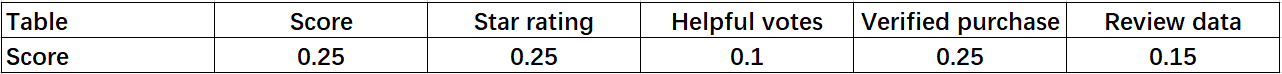
\includegraphics[width=.6\textwidth]{weight.png}
\caption{Weight}\label{fig:weights}
\end{figure}

\begin{figure}[!htbp]
\centering
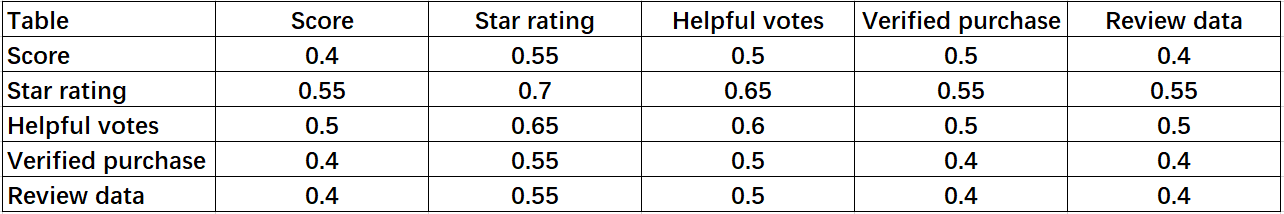
\includegraphics[width=.6\textwidth]{z1.png}
\caption{Fuzzy Consistency Matrix}\label{fig:Fuzzy Consistency Matrix}
\end{figure}

After passing the consistency check, we calculate the weight of each index based on matrix B. Based on experience, to improve the resolution of the results, we choose $\alpha=\frac{n-1}{2}$.

\begin{equation}\label{eq:1}
w_i = \frac{1}{n} - \frac{1}{2\alpha} + \frac{1}{n\alpha} * \sum\limits_{k=1}^n a_{ik} \quad i=1,2,3...,n
\end{equation}

From above results, it can be observed that Score, Helpful votes and Verified purchase are more informative than the other two. Sunshine Company should concern more about these indexes.


In addition, if these reviews need to be further processed, we can rank them using the method based on the weighted gray correlation degree. Then, informative reviews should be placed in a more prominent position. In this way, consumers can get product information faster, which is likely to help improving shopping experience increasing sales.



\subsection{Time-based Model}

\subsubsection{Forecast using SARIMA Model}
 Among all the features of the data, sales volume is one of the most important one. Therefore, we must pay attention to those most popular products. Due to the fact that most products in the dataset have only one or two sales amount and we can not analyze such a great number of products, we select the five most popular products in each category with a total number of 15 product. Then we use SARIMA to fit the history data and forecast the time series with 24 months horizon. Since there are lots of products taking on a seasonal sale amount feature, we use SARIMA instead of ARIMA model.\cite{3}
 
\begin{equation}
SARIMA : (p, d, q) (P, D, Q)_m
\end{equation}


\begin{equation}
y_{t} = c + \phi_{1}y_{t-1} + \cdots + \phi_{p}y_{t-p}
       + \theta_{1}\varepsilon_{t-1} + \cdots + \theta_{q}\varepsilon_{t-q} + \varepsilon_{t}
\end{equation}
$c$ is a constant, $\phi_i$ and $\theta_i$ is parameters, $y_i$ is history series and $\varepsilon_i$ is white noise, $i={1,2...}$  

  In our model, to show a better performance, we choose month period, thus we have $m=12$. We define $B$ as the backshift, then SARIMA $(p, d, q) (P, D, Q)_{12}$,:

  $$
  (1 - \phi_{1}B)~(1 - \Phi_{1}B^{12}) (1 - B) (1 - B^{12})y_{t} =  (1 + \theta_{1}B)~ (1 + \Theta_{1}B^{12})\varepsilon_{t}.
  $$

In order to make the best forecast with the data given by Sunshine Company, we search for optimal parameters (p, d, q) and (P, D, Q) from (0, 0, 0) to (3, 3, 3) step by step and select the parameter with the least AIC result. 

Figure \ref{fig:Forecasting ARIMA} shows the top 5 each product category by sales amount. The blue line is history sales data provided by Sunshine Company and the orange line is our forecasting result within 24 months(2 years). The slight yellow straight line at the bottom is the corresponding star ratings. From our result we can conclude that if the product sales amount remains high enough in recent years, the product also has potential to stand out in the future. However, trend is also an important factor. For instance, "NO.5 hair dryer" is popular in recent years but the trend is declining, so in our model we predict that this product will not remain succeeding in about 5 years. Therefore, for a newborn online E-commerce company, it is unwise to sell this product in the future. 

\begin{figure}[H]
\centering
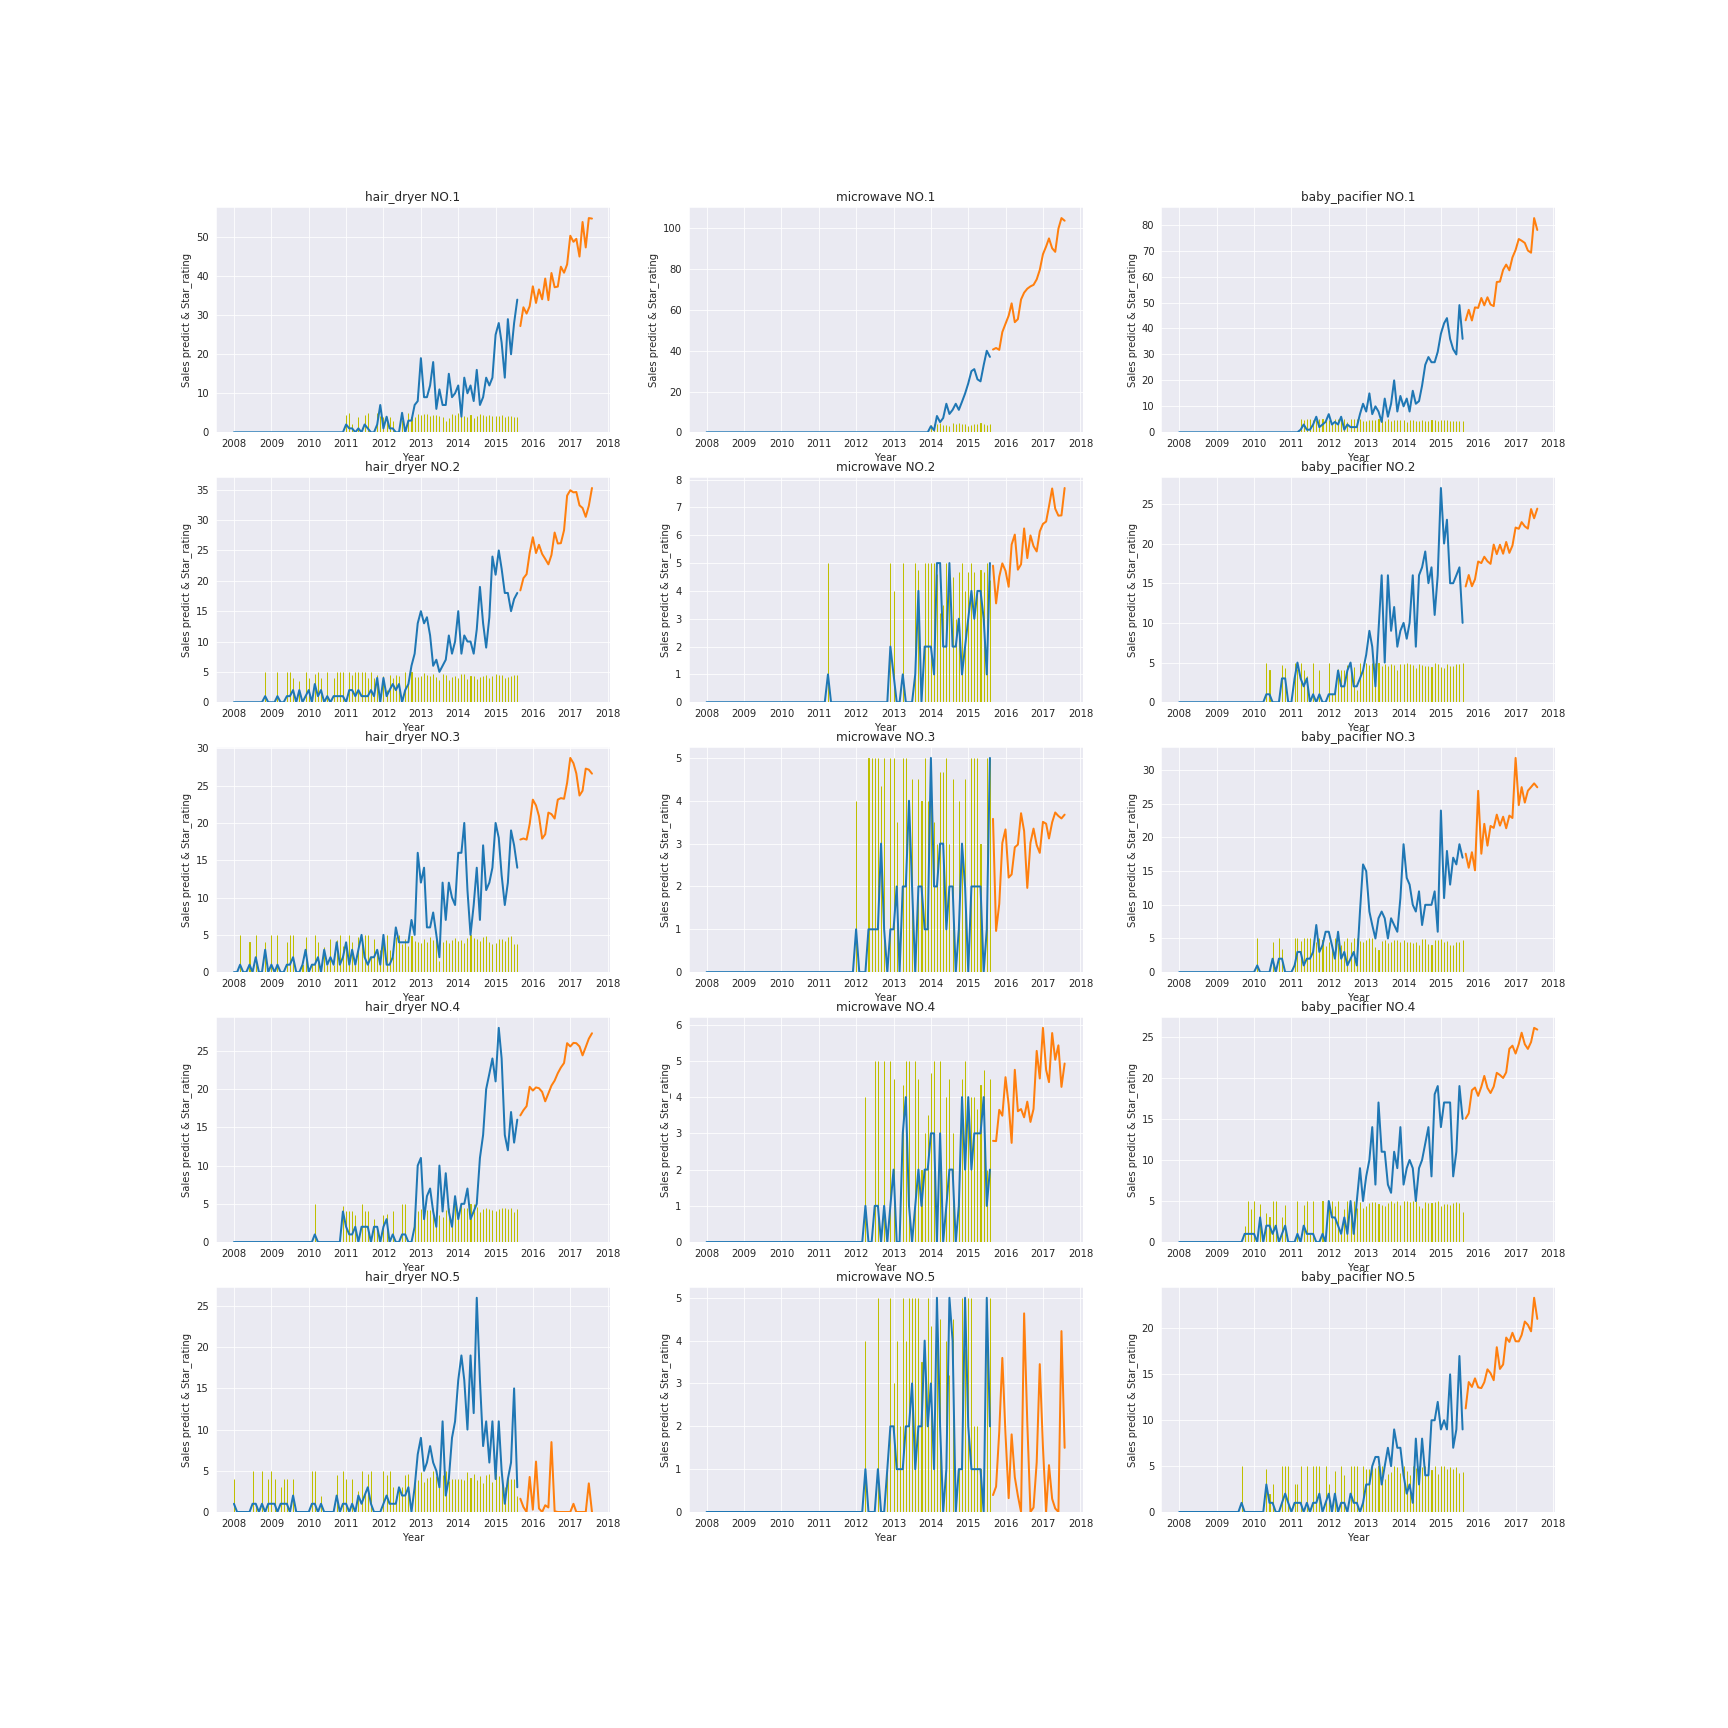
\includegraphics[width=0.9\textwidth]{Forecasting_ARIMA .png}
\caption{Forecasting with SARIMA}\label{fig:Forecasting ARIMA}
\end{figure}



\subsection{Text Mining about Reviews}
\subsubsection{Parsing Reviews with Dependencies Representation}

Dependencies representation aims at parsing sentences into several parts with word units and generating dependencies between words based on grammatical relationships. The words dependencies is manually categorized into more than 50 types. In addition, the model gives each word an attribute such as noun, adjective in the form of 'NOUN', 'ADJ' \cite{4}. In that way, we can filter the key information in the review text. For example, this is a review sentence of microwave: "This is the best standard blow dryer on the market". We generate a sentence dependency like this:

\begin{figure}[H]
\centering
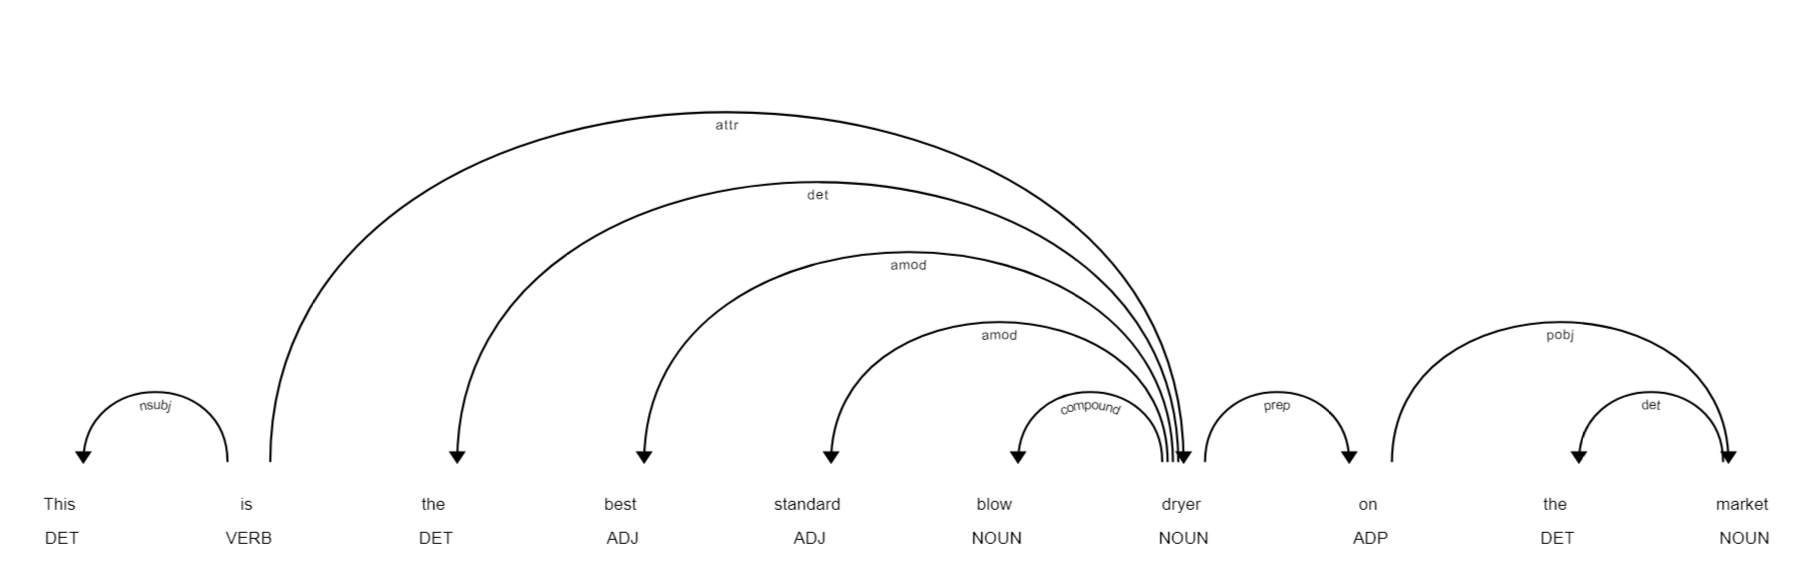
\includegraphics[width=.8\textwidth]{Stanford.png}
\caption{Sentence Dependencies Representation}\label{fig:sentence}
\end{figure}

\subsubsection{Word Frequency Statistics}
According to the "word dependency map", now we can count the top frequency word in the review. In our paper, we consider customers who make one, two or three star ratings are likely to make negative reviews, and customers who make four or five star ratings are likely to make positive reviews. Under this circumstances, we add up the total word frequencies and show them as follows:
\begin{figure}[H]
\centering
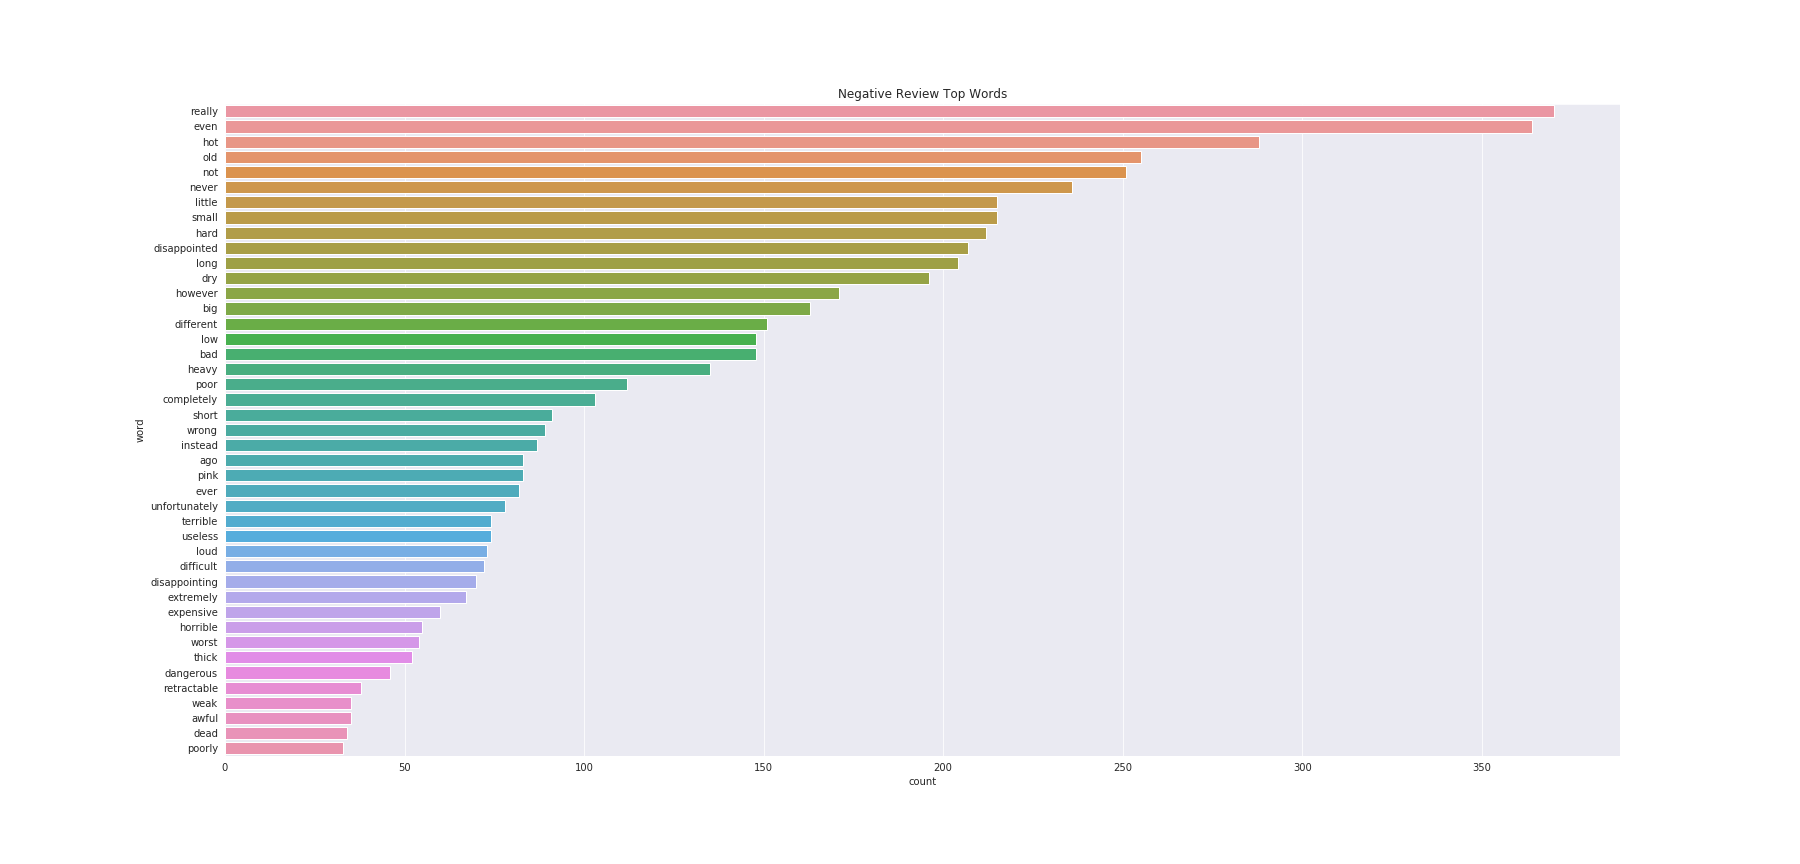
\includegraphics[width=.9\textwidth]{negative_word.png}
\caption{Top Negative Words}\label{fig:negative}
\end{figure}
\begin{figure}[H]
\centering
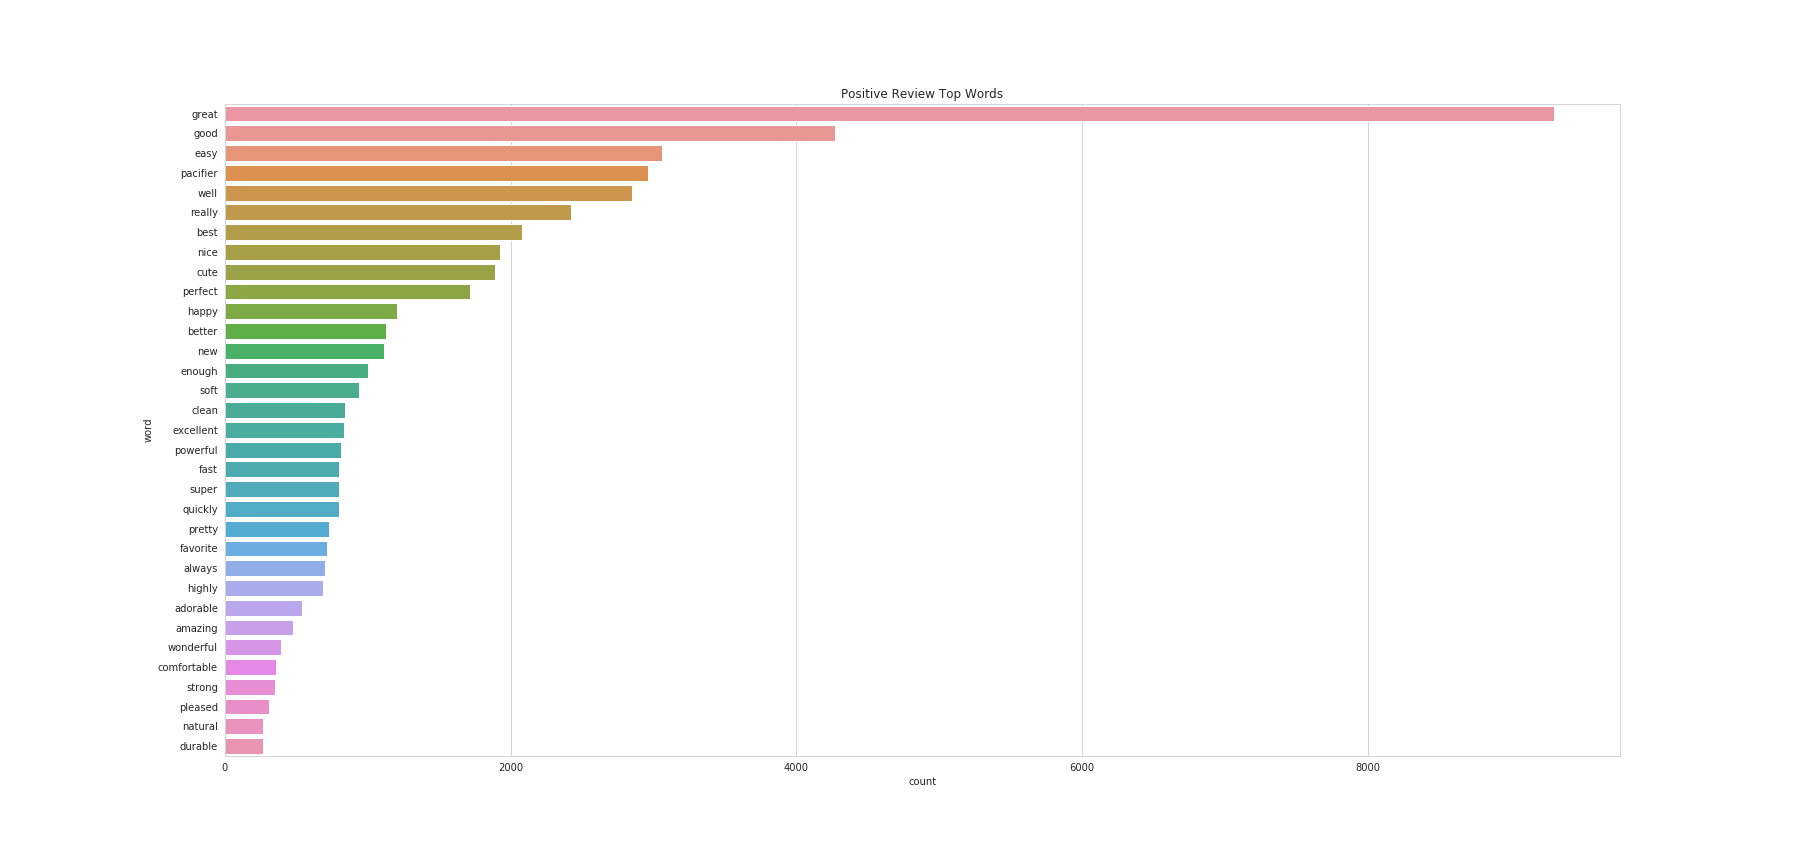
\includegraphics[width=.9\textwidth]{positive_word.png}
\caption{Top Positive Words}\label{fig:positive}
\end{figure}

In Figure \ref{fig:negative} and Figure \ref{fig:positive}, we illustrate several top words in both positive and negative reviews separately. It shows that positive words such as 'great', 'perfect', 'excellent' are most likely to appear in positive reviews, and words including 'bad', 'disappointed' and 'unfortunately' are most probable to be found in negative reviews.  At the same time, it is not surprising to find some words which do not have exact meanings such as 'really' appear both in positive and negative in a high frequency. However, we found some sligtly negative words also show high frequencies in positive reviews. Now we analyze this in detail. 

\begin{figure}[!htbp]
\centering
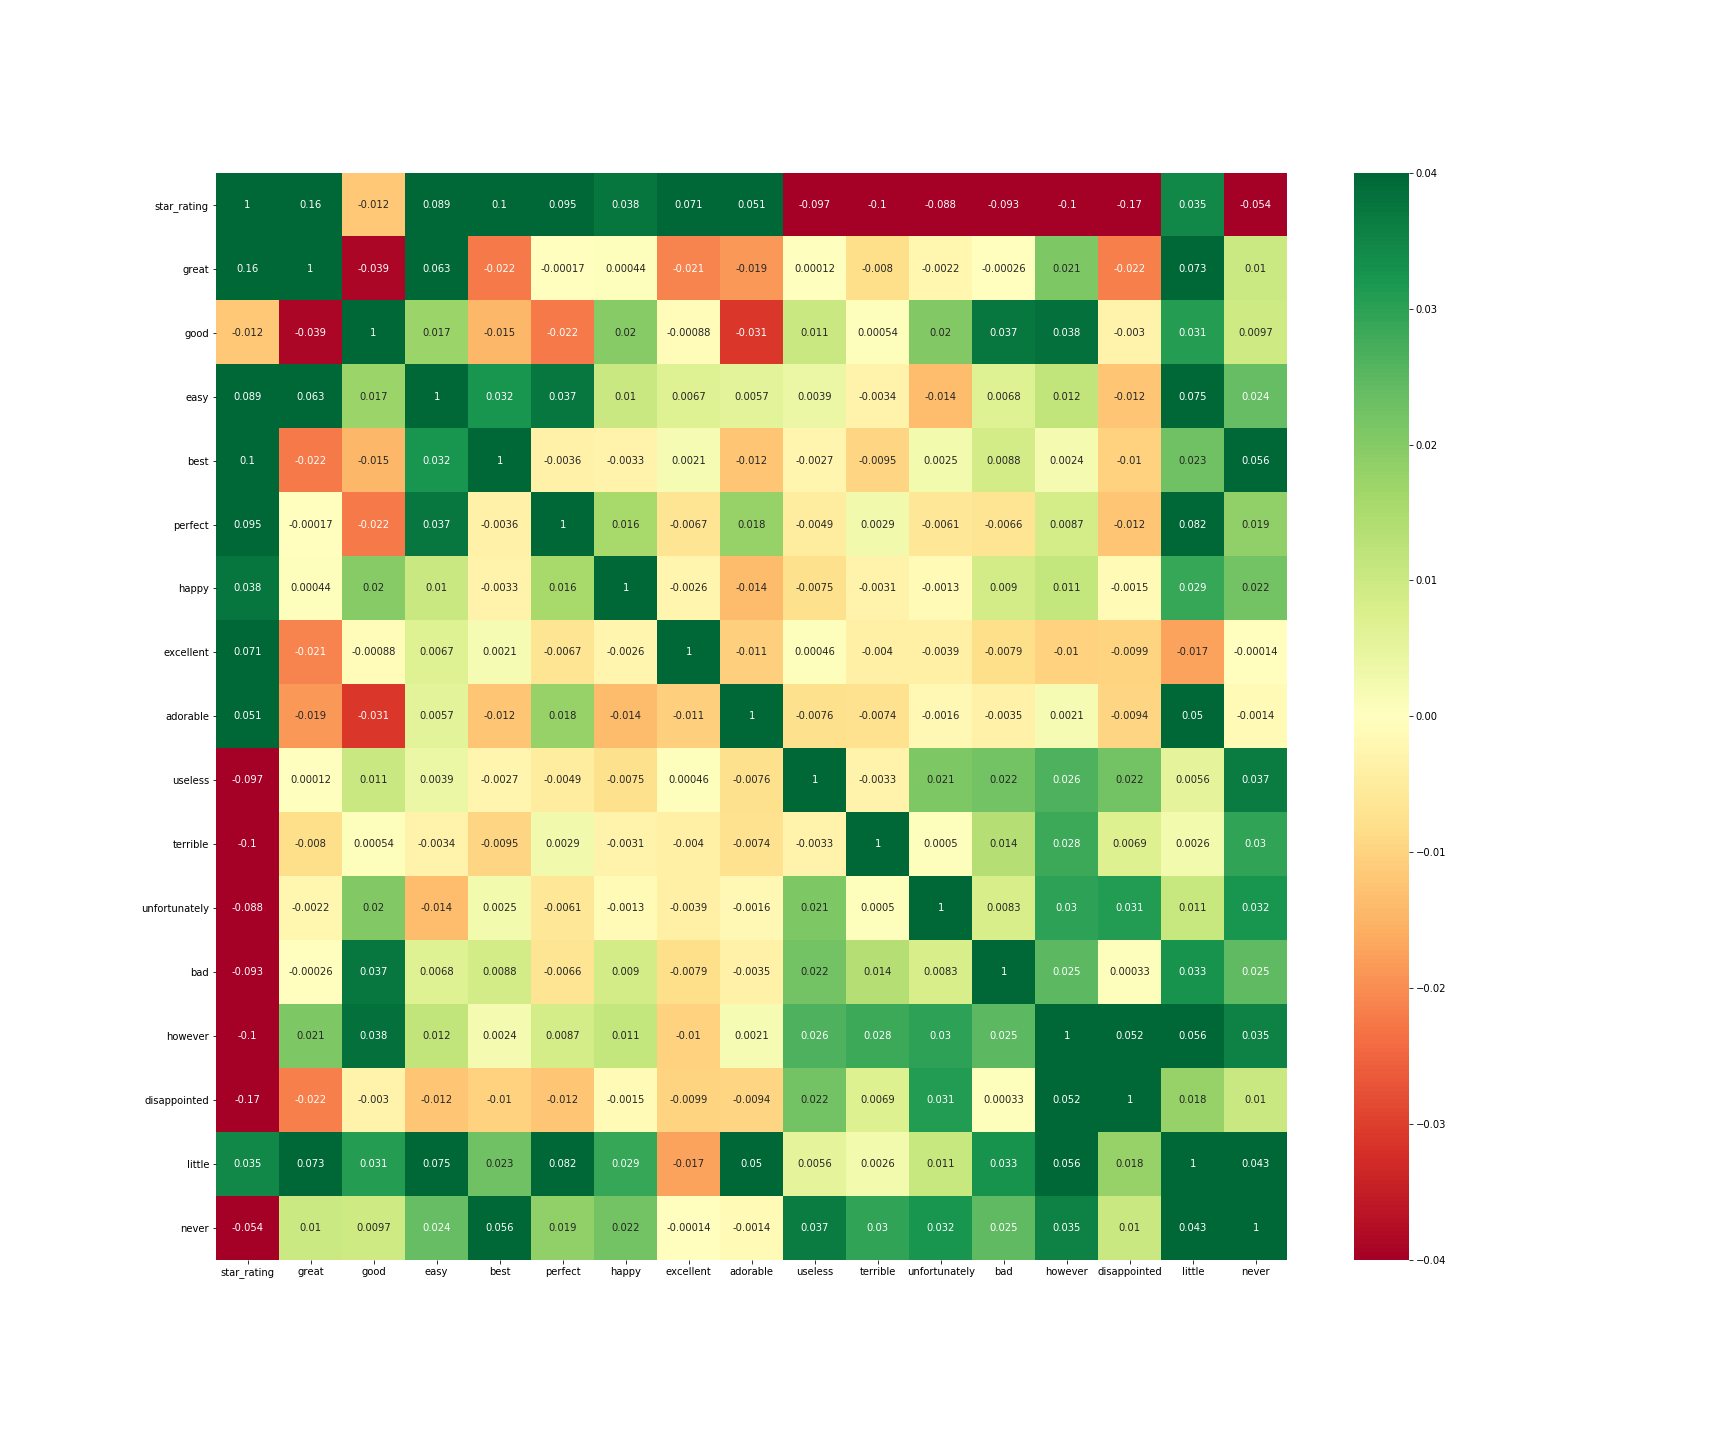
\includegraphics[width=.9\textwidth]{heatmap.png}
\caption{Covariance Matrix with High-Frequency Words}\label{fig:heatmap}
\end{figure}

Figure \ref{fig:heatmap} is a heatmap showing the covariance matrix of several top-frequency positive and negative words. In this map, we select \textbf{'great', 'good', 'easy', 'best', 'perfect', 'happy', 'excellent', 'adorable'} as typical positive words, and select \textbf{'never', 'little', 'disappointed', 'however', 'bad', 'unfortunately', 'terrible', 'useless'} as typical negative words. The first row and first column is the corresponding star rating. Obviously, the upper left corner and lower right corner takes on more "green color", meaning that the covariance between positive words vectors and the covariance between negative words vectors are larger, which tally with our intuition. In the heatmap, we can also figure out that the covariance between negative words(lower right corner) is slightly larger than the covariance between positive words(upper left corner), meaning that using negative words to predict a bad performance has more confident than using positive words to predict a good performance.

\subsubsection{Relationship Between Word Frequency and Star Rating}
From our intuition, there is also a great probable relationship between word frequency in a single review and star ratings.  For instance, if one customer comments "This microwave is bad" and the other customer comments "bad! bad! bad!", then we are confident to judge that the second customer is likely to give a lower star rating. To prove that, in this section we select several top-frequency words both in positive and negative words. The result is as follows:

\begin{figure}[H]
\centering
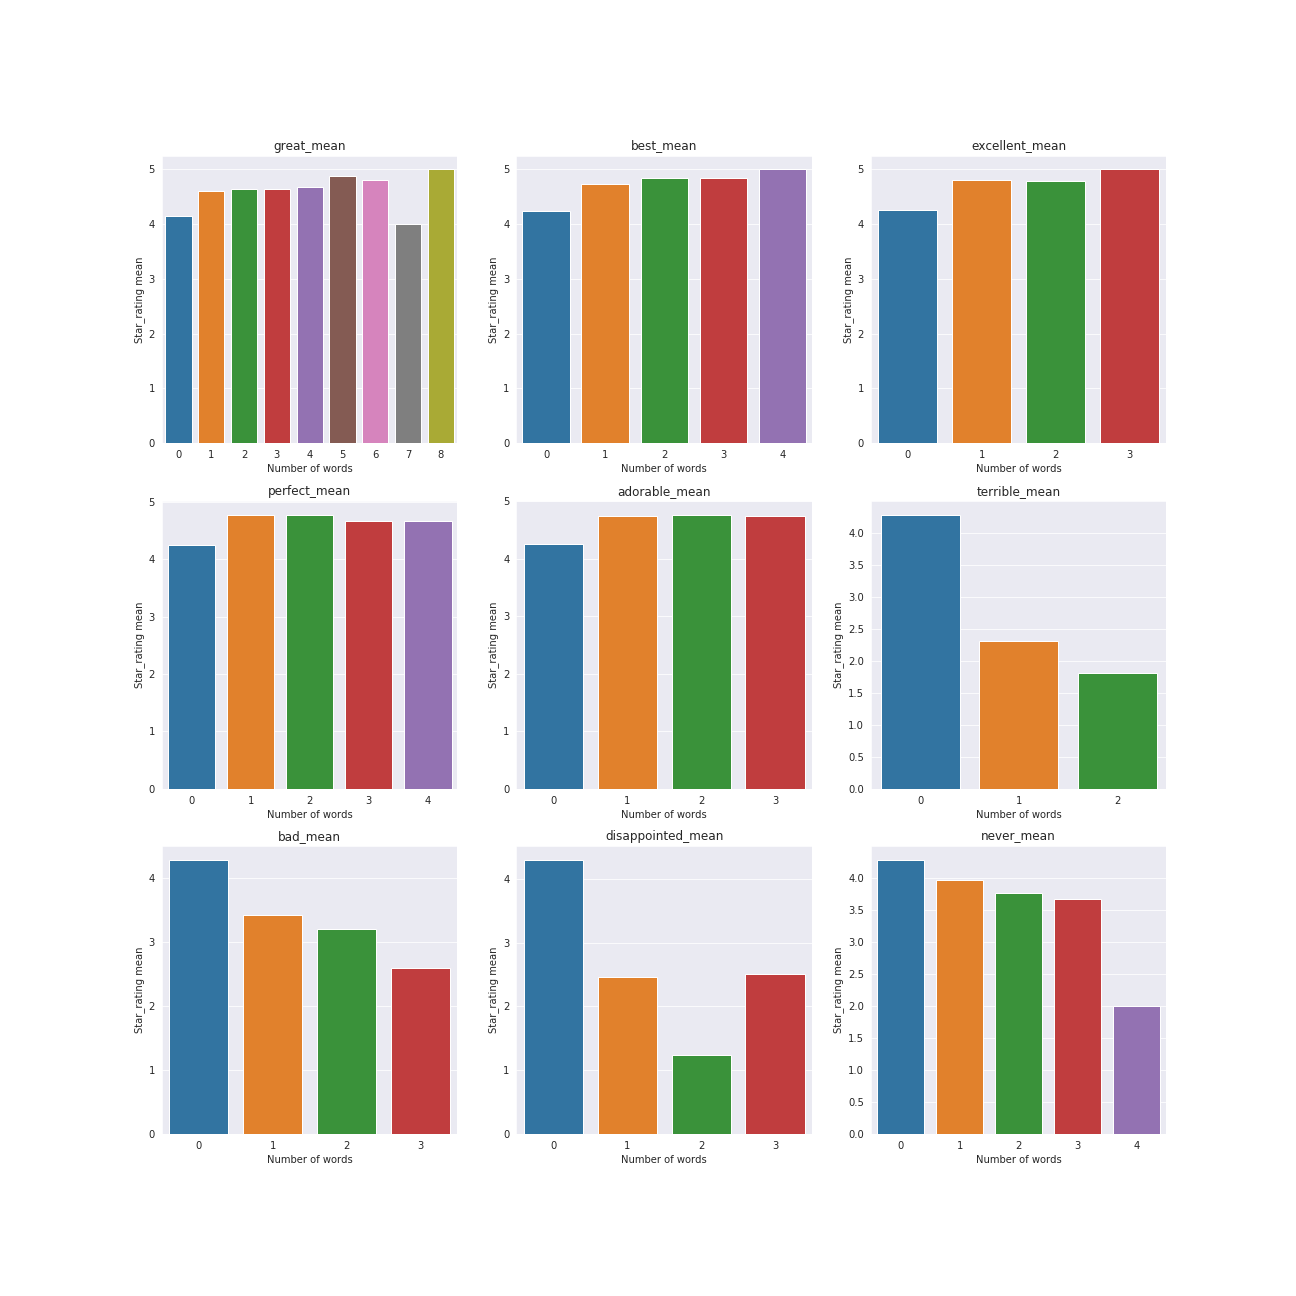
\includegraphics[width=.7\textwidth]{3_3_topwords_mean_score.png}
\caption{Relationship Between Word Frequency in single review and Star Rating}\label{fig:score}
\end{figure}

It is obvious that if there are more positive/negative words in a single comments, the customer is more likely to give a higher/lower star rating. But there are still some outliers, indicating that this rule is valid only when there is enough rating data.



\subsection{Combination of Star Rating and Review}
In our analysis above, we only use star ratings and reviews separately. However, this may not work well sometimes because in some online E-commerce platforms, the merchant may make a great number of fake purchase and give a five-star rating so as to attract customers. In this way the score is not real and our customer will be cheated. In order to tackle this problem, we combine the star rating and review score in a dynamic weights trained from helpful votes and total votes and generate a "Predict Score". This way we not only get an accurate result but also achieve a real-time evaluation to a new product. Just imagining the online sales situation in which it is impossible for the company to obtain enough helpful votes and total votes for a new product, so this combination is of great significance. 

 The detail can be described by equation \eqref{eq:1}\eqref{eq:2}:

\begin{equation}\label{eq:1}
Score\_weight = \frac{h_v}{t_v} * \frac{t_v-min(t_v)}{max(t_v)-min(t_v)}
\end{equation}

\begin{equation}\label{eq:2}
Predict\_Score = \frac{\sum{Score\_weight * Score}}{\sum{Score\_weight} }
\end{equation}

To achieve this combination, first we use NLTK VADER lexicon Structure to generate a polarity ranging from [-1,1] of each sentence. Then we rescale the polarity by function $f(x)=2x+3$ to [-5,5]. We consider this score to be the Review Scores. 

Next, we will determine the weight between and star ratings and Review Scores. In our model, we use Exhaustive Grid Search to search the weights. The search step is 0.01 from 0.01 to 1.00. Besides, We minimize Mean Square Error(MSE) to find the optimal hyperparameters.\cite{5}

\begin{gather}
\text{MSE}(y, \hat{y}) = \frac{1}{n_\text{samples}} \sum_{i=0}^{n_\text{samples} - 1} (y_i - \hat{y}_i)^2.\\
y_i = w_1 * Star\_Rating + w_2 * Review\_Score\\
\hat{y}_i = Predict\_Score\\
w_1+w_2=1
\end{gather}

Figure \ref{fig:MSE} shows the best weights to combine star ratings and review scores trained by history data. For the given sales data, the best weight parameters are as follows:

\begin{figure}[!htbp]
\centering
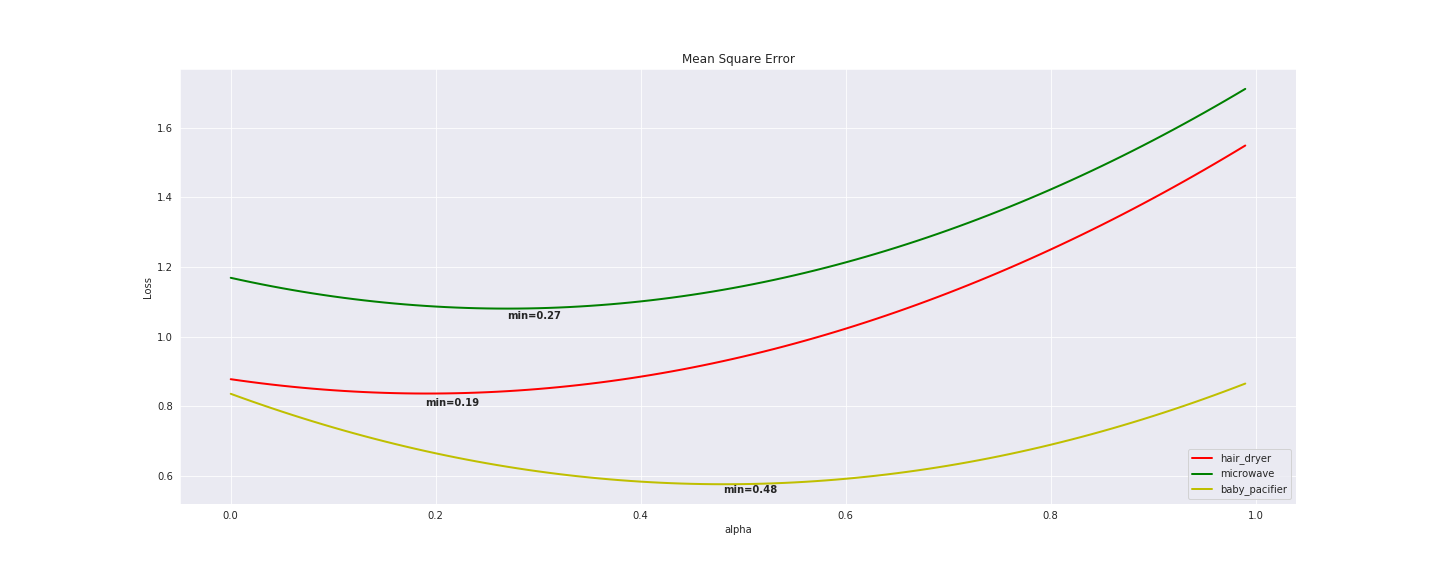
\includegraphics[width=.9\textwidth]{alpha_loss.png}
\caption{MSE}\label{fig:MSE}
\end{figure}

\begin{center}
\begin{tabular}{|c|c|c|}
\hline 
Product & Weight of Star Rating & Weight of Review Score\\
\hline  
hair dryer & 0.19 & 0.81\\
\hline
microwave & 0.27 & 0.63\\
\hline
baby pacifier & 0.48 & 0.52\\
\hline
\end{tabular}
\end{center}
From this tabular, we learn that star ratings are not always reliable. To generate a real score for the product, we must take reviews into consideration. 

\subsection{Model Refinement with ABSA}
Aspect Based Sentiment Analysis(ABSA) is a classical method in fine-grained level mainly focusing on detection of sentiments to all entities in a single sentence or paragraph. This will help the company to judge on which aspect should be revised if and why the customer give a high or low star rate\cite{6}. For example, if a customer write a comment "The logistics service is good and the hair dryer is cheap, but the sound too loud which is terrible.", then we will make a judgment that our service and dryer is good and there are some problems with the sound. In most circumstances, the customers probably give our product a lower star rating just because one some blemish. So our task is to find those some faults especially the mistakes due to our company's service.

\begin{figure}[!htbp]
\centering
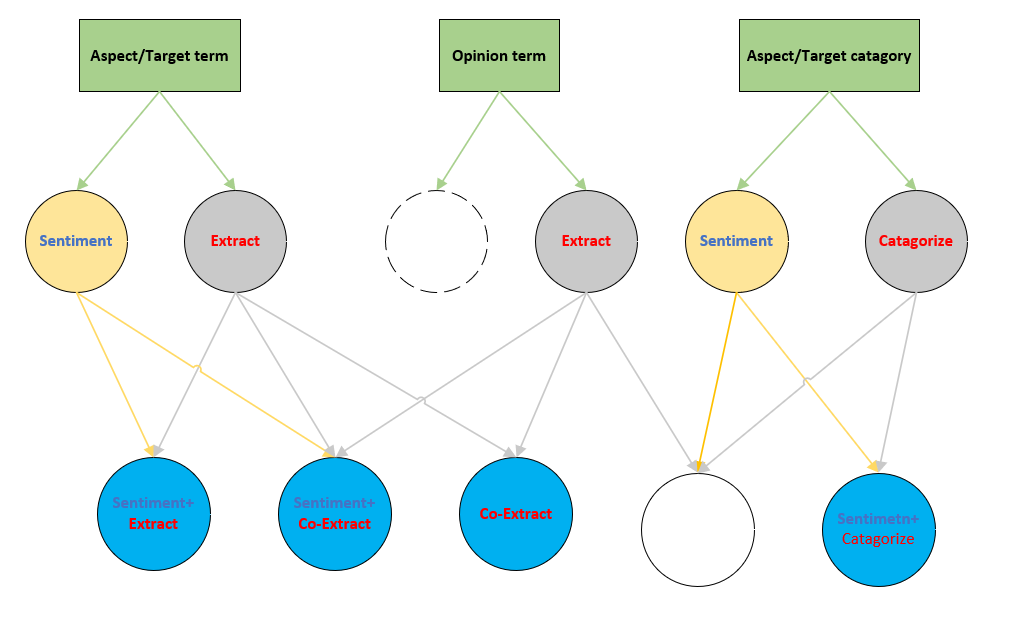
\includegraphics[width=.7\textwidth]{j.PNG}
\caption{ABSA Model}\label{fig:ABSA Model}
\end{figure}

Figure \ref{fig:ABSA Model} shows the basic architecture of Aspect Based Sentiment Analysis Model. The upper level consists of three object: aspect term, opinion term and aspect category. Aspect term is the entity we intend to evaluate; opinion term is the attitude to the entity and finally we categorize all aspect to make further conclusion. The steps are:

\begin{itemize}
\item Extract all entity expressions in the document set, and classify or group synonymous entity expressions into entity clusters.
\item Extracts all aspects representation of entities and classifies them into clusters. These aspects can be explicit or implicit.
\item Extract viewpoint holders from text or structured data to obtain and classify points of view.
\item Extract comment time and standardize different time formats
\item Determine whether an aspect is positive, negative, or neutral, or assign a digital emotional rating to that aspect.
\end{itemize}

We finish some preliminary ABSA modeling and the conclusion is:
\begin{itemize}
\item For hair dryer, most customers complain about the aspects including installation, noise, low speed, not powerful and quality of cord.
\item For microwave, what the customers complain most is the door. Besides, heat and service is also included 
\item For baby pacifier, we do not find obvious common problems. Probably because the baby cannot comment itself and there are a variety of pacifier types. Analyzing specific kind of products may conclude clearer result. 
\end{itemize}
By categorizing the aspects in our customer's reviews, we will have more specific target about what should be paid more attention when deciding whether to sell a product. For example, check the noise and power of a hair dryer or carefully examine the door's quality when importing the microwaves will definitely increase the customers' rating to our company and our product. 

\section{Discussion}
\subsection{Specific Rating Level \& Review}
In order to observe the impact of a specific star rating on reviews, we divide reviews into positive reviews and negative reviews through sentiment classification. We randomly select five products from each category, and we choose following four variables:
\begin{enumerate}[\bfseries 1.]
    \item Total number of positive reviews
    \item Total number of negative reviews
    \item Average star rating for positive views per month
    \item  Average star rating for negative views per month
\end{enumerate}
\begin{figure}[!htbp]
\centering
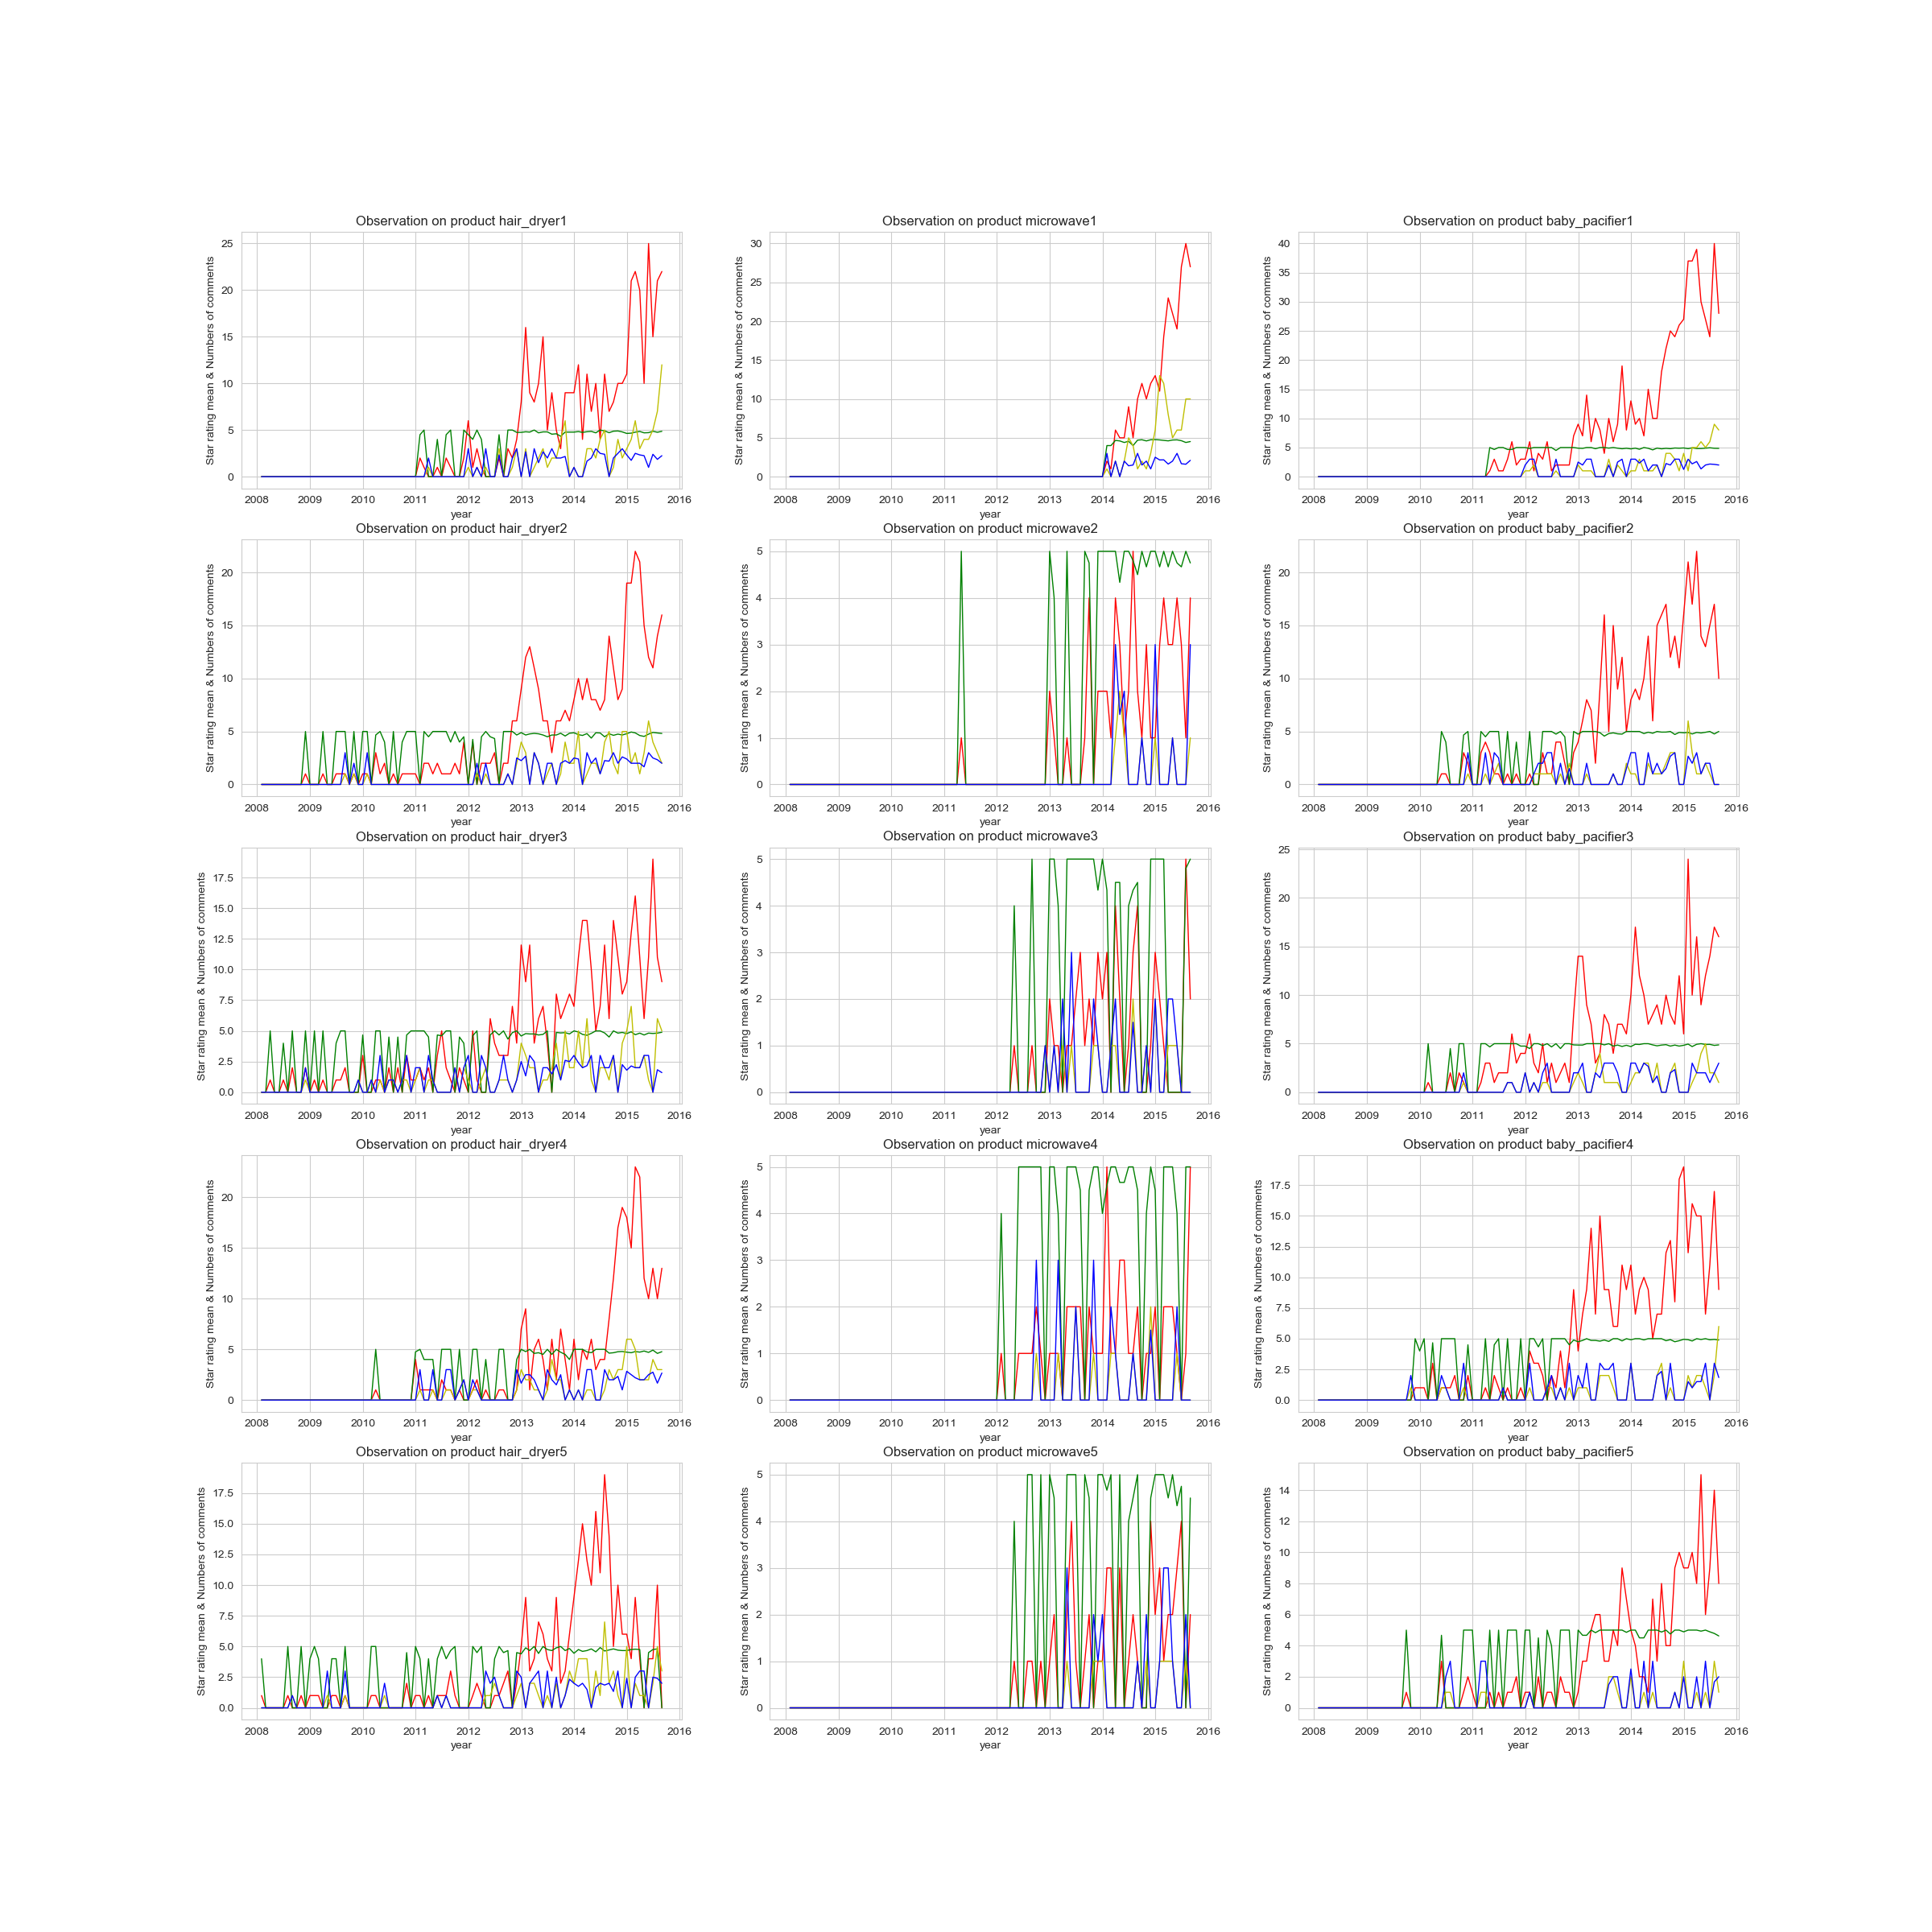
\includegraphics[width=0.9\textwidth]{2_D.png}
\caption{Observing impacts of specific star ranking }\label{Observing impacts of specic star ranking}
\end{figure}


Intuitively, we can speculate that there is a significant correlation between continued high star ratings and increasing positive comments. In addition, the average star rating of negative reviews fluctuates smoothly and randomly, and the number of negative reviews fluctuates only within a small range.
In order to verify our guess, we have processed the difference on numbers of reviews and. We can see that the number of positive reviews has achieved a steady trend, while the number of negative reviews has not changed significantly compared to the original image. Therefore, it can be considered that after a series of high star ratings, customers are more likely to write positive reviews, while negative star ratings are only related to the their personal situation such as shopping experience or product satisfaction, which will not trigger more reviews.

\begin{figure}[!htbp]
\centering
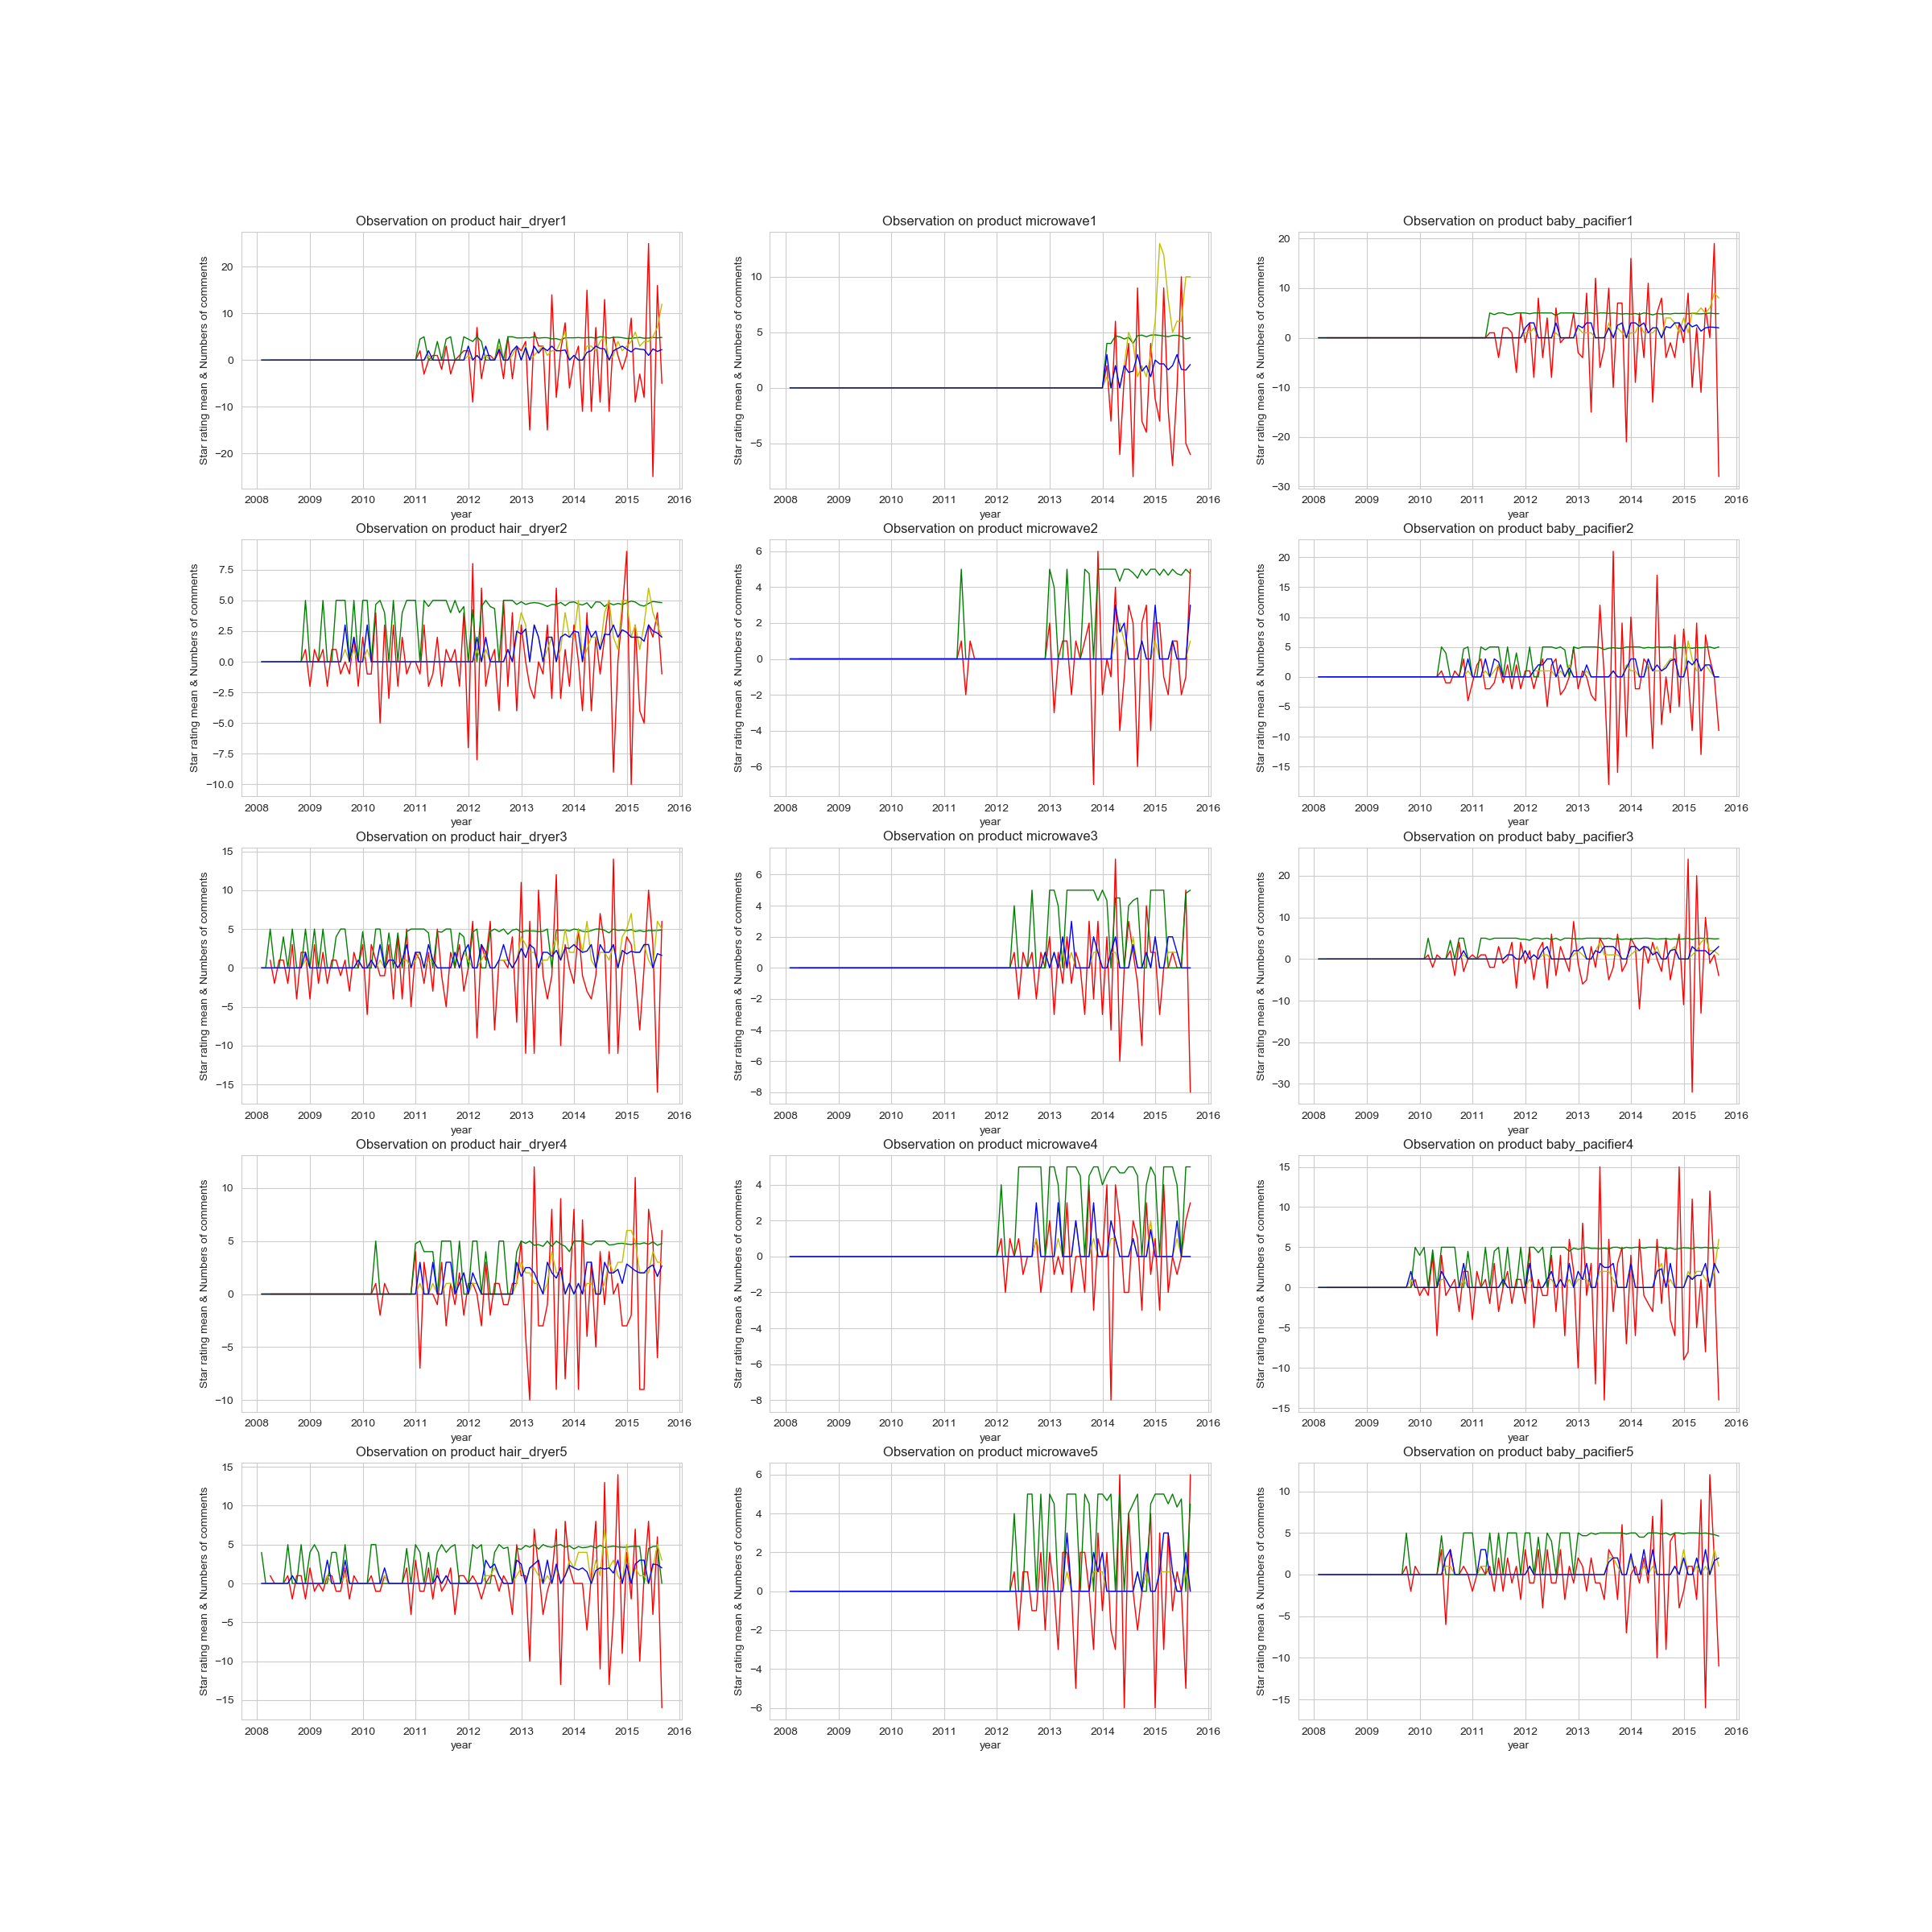
\includegraphics[width=0.9\textwidth]{2_D_diff_2.png}
\caption{Second-order difference}\label{Second-order difference}
\end{figure}

\subsection{Specific Text-based quality description \& Rating Level}
According to Figure\ref{fig:negative} and Figure\ref{fig:positive}, we can see that positive words  tend to appear with high star ratings, while negative words and adversative conjunctions tend to appear with low ratings. Besides, it's logical that some neutral words appear frequently in both ratings. 

According to Figure\ref{fig:heatmap}, we can see that the covariance between the positive words vectors and the covariance between the negatives words vector is larger, which quantitatively explains the specific quality descriptors of the text-based reviews are significantly related to the rating level.


\section{Sensitive analysis}

\subsection{Weights of star rating and review}
In the model of the combination of star rating and review, we change the weight of star rating and review and analyze the loss function's values.Just as shown in Figure \ref{fig:MSE}. The loss function's values fluctuate within a small range  as the weights change within 0.1 around optimal value, which verifies our model's robustness. But when the Star rating's weight goes up, function's values increase rapidly, model comes to an unstable state.


\section{Conclusion}

In our paper, We have done a lot of processing on the data. We extract expected data features from the raw data and study the relationship between them and the impact on product sales and prestige are studied, and a basic model and a time-dependent model are built on this basis.

Besides, our model also has strengths and weaknesses.
\subsection{Strengths}
\begin{itemize}
    \item Integrity. We have a thorough understanding of the requirements of the topic, and make full use of the data provided to build the model, making the model more reliable.
    \item Highly explicable. We use some classical and explcable methods, including fuzzy analytic hierarchy process, SARIMA, ABSA, etc.
    \item Extensibility. Our model discusses product reputation and uses “Predictive Score” to evaluate products. For the fact that helpful votes and total votes can not be obtained in time, the "Score" is only related to star ratings and reviews. In the future, if there is related research, more parameters can be introduced for more detailed and in-depth evaluation.
\end{itemize}

\subsection{Weaknesses}
\begin{itemize}
    \item Lack of necessary data supply. Less data means less features. The data features we extracted for our model's construction is not abundant enough, as a result, our model doesn't have strong robust.
    \item Subjective decision making method. In some places where different modeling methods need to be compared and discussed, we did not have enough time to discuss them in detail, and directly chose the method we judged to be more suitable for the current modeling requirements to discuss the problems to be solved. This makes it possible for us to pass by with better models.
 \end{itemize}

\section{Future Work}
Due to time constraints and our current shallow knowledge, there are still many shortcomings in our model. Future research work can be further studied from the following aspects.
\begin{itemize}
    \item Introduce more complicated deep model such as Dilated-RNN, DeepAR, and Bi-LSTM to enhance the accuracy of text comprehension and time series forecasting.
    \item There are lots of variation and refinement about ABSA model, and it can be combined with some deep learning method to accomplish an End-to-End real-time sentence evaluation. 
    \item Use Pre-train model such as "Bert" to enhance the speed of training.
    \item Use more recent data to do cross validation and further testing for our model.
\end{itemize}


% 以下为信件/备忘录部分,不需要可自行去掉
% 如有需要可将整个 letter 环境移动到文章开头或中间
% 请在后一个花括号内填写信件(Letter)或备忘录(Memorandum)标题
\begin{letter}{Letter}
\begin{flushleft}  % 左对齐环境,无首行缩进
\textbf{To:} Sunshine Company Marketing Director\\
\textbf{From:} Team 2020987\\
\textbf{Date:} March $10_{th}, 2020$\\
\textbf{Subject:} A suggestion for a new product marketing strategy
\end{flushleft}

We are glad to hear that you are looking for a diverse range suggestions in order to make new products more popular. In this letter, we will briefly introduce our research and analysis of the previous products' datasets. Based on these, we recommend the optimal online sales strategy after we balanced our consideration. In addition, through research on the design of well-sold products, we found several design features that can effectively improve users' satisfaction.

At first, we made a preliminary comparison of importance of the index of the review:"Helpful votes","Star rating","Verified purchase" and "Review Date". The result showed that Helpful votes","Star rating" and "Verified purchase" are more worthy to be studied, namely, play a significant role in the research of products.

Then, we discussed the future potential tendency of the products' popularity. Through a comprehensive analysis of product data from 2008 to 2015, we find that products with higher star ratings and higher sales volume have great potential performing better in the future.

%Afterwards, We analyzed the polarity of the reviews

%Lastly, We have established a product scoring system for product evaluation based on the %previous index (star ratings, helpful votes, total votes and reviews), Futhermore, we %distcarded both helpful votes and total votes to  construct a real time evaluation model. 

Based on our analysis, we'd like to provide some suggestions on your products' online sales strategy and design features.

\begin{enumerate}
    \item We recommend that your company concern more about recent data, and give priority to products with high sales and positive reviews in the past few years.
    \item We suggest that the production scale of products with large sale fluctuations which may cause huge loss should be considered cautiously. You can periodically adjust the sale scale based on real-time situation.
    \item We recommend that when evaluating products, you are supposed to pay more attention to specific review content and reduce the proportion of star ratings in your evaluation. This is because we find that specific review contents, such as the extreme negative words and adversative conjunctions, somtimes are more important than star ratings through the "Predict Score". Therefore, we suggest your company place the most informative reviews in a prominent place on your online platform to help your customers make correct judgements.
    \item We suggest that before your company place a product online, you had better examine the aspects that most customers are complaining about. For example, the noise of the hair dryer and the quality of microwave door. We believe the details will provide your customers better service.
\end{enumerate}
Wish our suggestions can support you to make correct decisions and attract more customers in the future. We are very eager to receive your further query on our plan and looking forward to hearing from you.\\

\begin{flushleft}Yours sincerely,\\
A group of modelers\\\end{flushleft}
\begin{flushright}3/10/2020\end{flushright}


\end{letter}


% 参考文献,此处以 MLA 引用格式为例
\begin{thebibliography}{99}
\bibitem{1} Farooq, Umar, et al. "Product reputation evaluation: The impact of conjunction on sentiment analysis." 7th Int. Conf. Software, Knowledge, Information Management and Applications (SKIMA 2013)(Chiang Mai Thailand, 2013). 2013.
\bibitem{2} Jijun Zhang . Fuzzy Analytic Hierarchy Process (FAHP) [J]. Fuzzy Systems and Mathematics, 2000, 14 (2): 80-88
\bibitem{3} Seasonal ARIMA models.\emph{\url{https://otexts.com/fpp2/seasonal-arima.html}}
\bibitem{4} De Marneffe, Marie-Catherine, and Christopher D. Manning.Stanford typed dependencies manual.  Technical report, Stanford University, 2008. 
\bibitem{5} Hutto, Clayton J., and Eric Gilbert. "Vader: A parsimonious rule-based model for sentiment analysis of social media text." Eighth international AAAI conference on weblogs and social media. 2014.
\bibitem{6} Li, Xin, et al. "A unified model for opinion target extraction and target sentiment prediction." Proceedings of the AAAI Conference on Artificial Intelligence. Vol. 33. 2019.
\end{thebibliography}
\end{document}  % 结束